\documentclass[10pt]{article}
\usepackage{icmlko}

\icmlmeta{IP 파운데이션 월드모델}{78}{아홉째는 평균을 안 건드리고 자만 좁혔다}{일본 만화를 넣으니 판정치가 그대로이고 반폭만 10퍼센트 줄었다 --- 그리고 교차점에 앉았다}

\begin{document}

\twocolumn[
\icmlheader

\begin{abstract}
노트 76이 배선을 닫았고 노트 77이 누출을 다 막았다. 남은 지렛대는 도메인
하나뿐이라 아홉째를 넣었다 --- \textbf{일본 만화 2,400건}(AniList 공개 GraphQL,
키 불필요). 축 배선을 웹툰과 \emph{일부러 같게} 맞췄다(태그 수 · 작가 이력 ·
성인 여부 · 연재 밀도). \textbf{판정치는 그대로다} --- 앙상블 $\rho$가
$+$0.3915에서 $+$0.3915. 대신 \textbf{반폭이 0.0446에서 0.0402로 10\% 줄었다}.
셀 수 법칙이 예측한 값이 0.0392이므로 거의 정확하다. \textbf{평균을 안 건드리고
자만 좁힌 첫 도메인}이다. 만화가 앉은 자리도 특이하다 --- 대상으로 $+$0.373,
출처로 $+$0.383으로 \textbf{둘이 거의 같다}. 아홉 중 유일하게 균형점이고,
상충 법칙의 두 직선이 교차하는 지점이다. 노트 74의 ``닮은 것이 특별하지 않다''도
\textbf{두 번째 사례를 얻었다} --- 웹툰과 만화는 라벨도 축도 같은 자리인데
쌍 이점이 $+$0.030 / $+$0.024다(게임/모바일은 $+$0.052 / $-$0.023이었다).
법칙은 아홉 점에서 $r=+$0.989다. 제품 수치도 갱신했다 --- 노트 77의 가장
엄격한 규약(과거 팝업 16건으로 공간을 만들고 새 기획을 하나씩)에서
\textbf{$\rho=+$0.5268 {[}$+$0.251, $+$0.717{]}}이다.
\end{abstract}
]

\begin{figure*}[t]
\centering
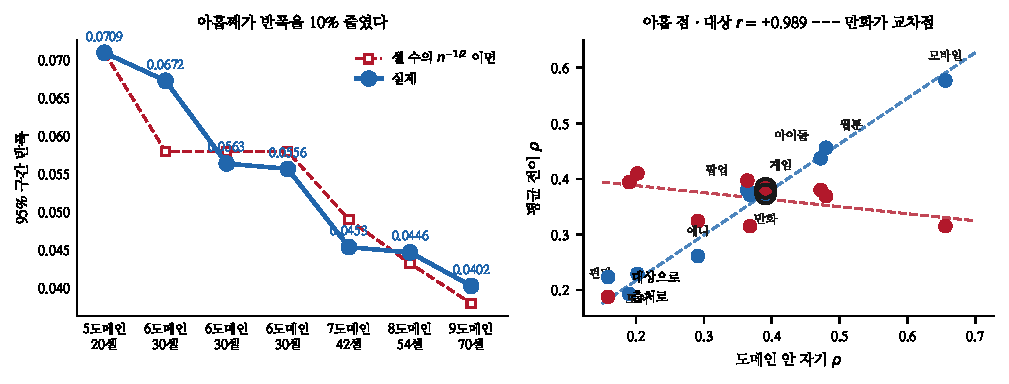
\includegraphics[width=\textwidth]{figs/ninth.pdf}
\caption{왼쪽 --- 구간 반폭의 이력. 오른쪽 --- 아홉 도메인의 두 법칙(테두리가 만화).}
\end{figure*}

\section{아홉째 도메인}

\begin{table}[t]
\centering\tsize
\caption{일본 만화. 축 배선을 웹툰과 같게 맞췄다.}
\begin{tabular}{lll}
\toprule
슬롯 & 만화 & 웹툰 \\
\midrule
라벨 & 서재 등록 수 & 관심 등록 수 \\
타깃 폭 & 태그 수 & 태그 수 \\
매장 노출도 & 작가 이력 & 작가 이력 \\
입장 허들 & 성인 여부 & 유료 여부 \\
굿즈 규모 & 연재 밀도 & 연재 밀도 \\
\midrule
표본 & 2,400건 & 2,817건 \\
공통 3축 관측 & 1,551건 & 2,817건 \\
시작 연도 & 1952--2025 & 2006--2026 \\
\bottomrule
\end{tabular}
\end{table}

노트 74에서 스팀/모바일에 같은 설계를 썼던 이유 그대로다 --- 배선이 같으면
두 도메인의 차이가 배선이 아니라 시장에서 온다. 표본은 인기순 상위 2,400건이라
스팀 topsellers · 앱스토어 차트와 같은 한계를 갖는다.

\section{평균은 그대로, 자만 좁아졌다}

\begin{table}[t]
\centering\tsize
\caption{구간 반폭의 이력.}
\begin{tabular}{lrrr}
\toprule
& 도메인 & 셀 & 반폭 \\
\midrule
노트 44 & 5 & 20 & 0.0709 \\
노트 68 & 6 & 30 & 0.0556 \\
노트 72 & 7 & 42 & 0.0453 \\
노트 75 & 8 & 54 & 0.0446 \\
\textbf{노트 78} & \textbf{9} & \textbf{70} & \textbf{0.0402} \\
\bottomrule
\end{tabular}
\end{table}

셀 수의 $n^{-1/2}$가 예측한 값이 $0.0446\times\sqrt{54/70}=0.0392$이고 실제가
0.0402다. \textbf{노트 69에서 세운 셀 수 법칙이 아홉 도메인에서도 맞는다.}

\claimx{도메인을 하나 더하면 반폭이 셀 수의 $n^{-1/2}$만큼 줄어든다 --- 다섯에서
아홉까지 일곱 측정에서 유지된다. 그리고 아홉째는 \emph{평균을 안 건드렸다}
($+$0.3915 그대로).}{평균이 그대로인 것은 만화가 우연히 전체 평균에 가까운
도메인이어서일 수 있다. 다음 도메인은 평균을 움직일 것이다.}

\section{만화는 교차점에 앉았다}

\begin{table}[t]
\centering\tsize
\caption{아홉 도메인 10,571건 · 70셀.}
\begin{tabular}{lrrrr}
\toprule
도메인 & $n$ & 자기 $\rho$ & 대상으로 & 출처로 \\
\midrule
모바일 & 1991 & $+$0.656 & $+$0.577 & $+$0.315 \\
웹툰 & 2817 & $+$0.480 & $+$0.456 & $+$0.369 \\
아이돌 & 62 & $+$0.472 & $+$0.437 & $+$0.380 \\
\textbf{만화} & \textbf{1551} & $+$0.391 & \textbf{$+$0.373} & \textbf{$+$0.383} \\
팝업 & 75 & $+$0.368 & $+$0.371 & $+$0.315 \\
게임 & 472 & $+$0.364 & $+$0.380 & $+$0.397 \\
애니 & 1420 & $+$0.291 & $+$0.261 & $+$0.324 \\
도서 & 242 & $+$0.202 & $+$0.229 & $+$0.410 \\
펀딩 & 400 & $+$0.190 & $+$0.193 & $+$0.394 \\
\midrule
\multicolumn{2}{l}{앙상블 판정치} & \multicolumn{2}{r}{\textbf{$+$0.3915}} &
$[+0.348, +0.428]$ \\
\multicolumn{2}{l}{자기 $\rho$와의 상관} & & $+$0.989 & $-$0.493 \\
\bottomrule
\end{tabular}
\end{table}

만화는 대상으로 $+$0.373, 출처로 $+$0.383이다. \textbf{아홉 중 유일하게 둘이
같다.} 상충 법칙의 두 직선(대상은 오르고 출처는 내린다)이 자기 $\rho\approx0.39$
근처에서 교차하는데 만화가 정확히 거기 있다.

\begin{quote}\fontsize{9.5}{11.5}\selectfont
\textbf{교차점에는 실용적 뜻이 있다.} 자기 상관이 그보다 높으면 대상으로 쓰고
출처로는 쓰지 마라(모바일 · 웹툰). 낮으면 출처로 쓰고 대상으로는 기대하지 마라
(펀딩 · 도서). 만화는 \emph{둘 다} 된다.
\end{quote}

\section{닮은 것이 특별하지 않다 --- 두 번째 사례}

\begin{table}[t]
\centering\tsize
\caption{표면이 닮은 두 쌍. 나머지 출처 평균과 비교.}
\begin{tabular}{lrrr}
\toprule
셀 & $\rho$ & 나머지 & 차이 \\
\midrule
만화 $\to$ 웹툰 & $+$0.482 & $+$0.452 & $+$0.030 \\
웹툰 $\to$ 만화 & $+$0.394 & $+$0.370 & $+$0.024 \\
\midrule
게임 $\to$ 모바일 & $+$0.601 & $+$0.548 & $+$0.052 \\
모바일 $\to$ 게임 & $+$0.364 & $+$0.387 & $-$0.023 \\
\bottomrule
\end{tabular}
\end{table}

노트 74가 스팀/모바일에서 본 것이 웹툰/만화에서 반복된다. 라벨도 축도 같은
자리인데 쌍 이점이 구간 반폭(0.040) 안에 있다.

\claimx{표면 유사성은 전이를 안 만든다 --- 두 쌍에서 반복됐다. 전이를 만드는
것은 자기 상관의 높낮이지 무엇을 파느냐가 아니다.}{두 쌍 다 배선을 일부러
같게 맞췄다. 각자 최적 배선을 찾았다면 이점이 생겼을 수 있다.}

\section{팝업과 제품 수치}

\begin{table}[t]
\centering\tsize
\caption{팝업을 맞히는 여덟 출처.}
\begin{tabular}{lrlr}
\toprule
아이돌 & $+$0.4762 & 게임 & $+$0.4451 \\
펀딩 & $+$0.4729 & 웹툰 & $+$0.3240 \\
\textbf{만화} & \textbf{$+$0.4559} & 모바일 & $+$0.2225 \\
도서 & $+$0.4497 & 애니 & $+$0.1239 \\
\bottomrule
\end{tabular}
\end{table}

만화가 셋째다. 팝업 앙상블은 $+$0.449로 그대로이고 대상 전이 평균이 $+$0.359에서
$+$0.371로 올랐다.

\begin{table}[t]
\centering\tsize
\caption{제품 수치. 노트 77의 규약 넷, 시점 2025 · 미래 59건.}
\begin{tabular}{lrr}
\toprule
규약 & 8도메인 & 9도메인 \\
\midrule
① 한꺼번에 & $+$0.5324 & $+$0.5294 \\
② 하나 빼고 & $+$0.5313 & $+$0.5294 \\
③ 과거 공간 & $+$0.5279 & $+$0.5251 \\
\textbf{④ 완전 한 건씩} & $+$0.5216 & \textbf{$+$0.5268} \\
\bottomrule
\end{tabular}
\end{table}

가장 엄격한 규약에서 $+$0.5268 {[}$+$0.251, $+$0.717{]}이다. 도메인이 하나
늘어도 제품 수치는 안 흔들린다.

\section{한계}

\begin{itemize}[leftmargin=1.1em,itemsep=0.15em]
\item 만화 표본에 \textbf{한국 작품 556건}이 섞여 있다(AniList가 웹툰을 MANGA로
      분류한다). 웹툰 도메인과 개념이 겹치는데 갈라 보지 않았다.
\item 라벨 범위가 좁다 --- 인기순 상위만 모아 $\log_{10}$ 3.72$\sim$5.52,
      SD 0.30이다. 다른 도메인은 SD가 0.5$\sim$1.3이다.
\item 굿즈 규모가 65\%만 관측된다(화수 결측). 공통 3축이 다 있는 것이
      2,400건 중 1,551건이다.
\item 미디어 투입 대응물이 없어 사실상 네 축이다.
\item ``평균을 안 건드렸다''는 우연일 수 있다. 한 도메인으로 본 것이다.
\end{itemize}

\section{다음}

\begin{enumerate}[leftmargin=1.3em,itemsep=0.15em]
\item 만화의 한국 작품 556건을 갈라 웹툰과의 관계를 다시 본다.
\item 열째 도메인 --- 셀 70$\to$90. 반폭 예상 0.0355.
\item 노트 74가 계산한 대로 후보 도메인의 \textbf{자기 상관을 먼저 재서} 고른다.
      교차점($\approx$0.39)보다 높은 것을 고르면 대상으로 좋고, 낮은 것을
      고르면 출처로 좋다.
\item 팝업 표본. 노트 75가 계산한 510건 전에는 팝업 기준 판정을 못 한다.
\end{enumerate}

\vspace{0.6em}
\hrule height 0.3pt
\vspace{0.5em}
{\footnotesize
\textbf{참고문헌}\\[0.3em]
Ben-David, S. et al. (2010). A theory of learning from different domains.
\emph{Machine Learning}, 79(1--2), 151--175.\\[0.15em]
Zamir, A. R. et al. (2018). Taskonomy: disentangling task transfer learning.
\emph{CVPR}, 3712--3722.\\[0.15em]
Standley, T. et al. (2020). Which tasks should be learned together in multi-task
learning? \emph{ICML}, 9120--9132.\\[0.15em]
Kish, L. (1965). \emph{Survey Sampling}. Wiley.\\[0.15em]
Efron, B., Tibshirani, R. J. (1993). \emph{An Introduction to the Bootstrap}.
Chapman \& Hall.
}

\end{document}
